\clearpage
\sffamily
{\bfseries\color[rgb]{0.4,0.4,0.4}
Regra 4 – Os Jogadores ('Equipamento')}
\phantomsection
\addcontentsline{toc}{subsection}{Regra 4 – Os Jogadores ('Equipamento')}

\bigskip

{\bfseries Segurança }

\headlinebox

Um jogador não deve usar equipamento ou vestir qualquer coisa que seja perigosa para si mesmo ou para outro jogador (incluindo qualquer tipo de joia).

\bigskip

{\bfseries O Design dos Robôs}

\headlinebox

Os robôs participantes das competições da Liga Humanóide devem ter um plano corporal semelhante ao humano, como mostrado na Fig. \ref{fig:bodyplan}. Eles devem consistir em duas pernas, dois braços e uma cabeça, que estão presos a um tronco.

\bigskip

Os robôs devem estar equipados com uma alça, para serem recolhidos com segurança e sem causar danos ao robô e ao manipulador. A alça deve ser facilmente acessível e não deve interferir com a operação do robô.

\begin{figure}[h]
\begin{center}
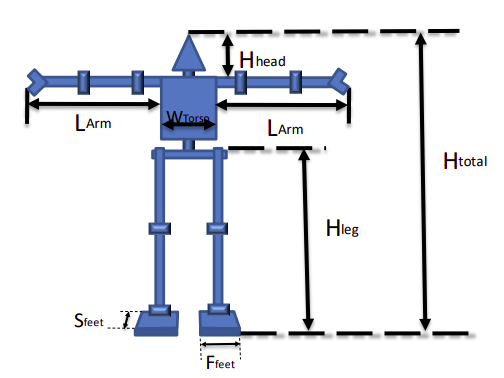
\includegraphics[width=0.7\textwidth]{img/bodyplan.png}
\caption{Exemplo de plano corporal de um robô humanóide}
\label{fig:bodyplan}
\vspace{-3ex}
\end{center}
\end{figure}


Os robôs devem ser capazes de ficar em pé e andar sobre as pernas.
Os únicos modos de locomoção permitidos são andar bípede, correr e saltar.

\bigskip

Todas as ações dos robôs devem ser cinematicamente equivalentes aos movimentos humanóides.

\bigskip

{\bfseries Altura do Robô}

\headlinebox

Com base em $H_{total}$, aplicam-se as seguintes restrições de tamanho:
\begin{itemize}
\item 25 cm ${\leq}$ $H_{total}$ ${\leq}$ 100 cm.
\end{itemize}

$H_{total}$ é definido como a altura do robô quando está em pé
(com os joelhos totalmente estendidos, cf. Fig. \ref{fig:bodyplan}).
$H_{total}$ é medido com a cabeça do robô orientada de tal forma que
está inclinado para o seu ângulo máximo de inclinação para cima ou para a linha do horizonte, o que for menor.

\newpage

{\bfseries Restrições de peso}

\headlinebox

Para a categoria Entry Level, não há restrições de peso. No entanto, como o objetivo da competição é incentivar a construção de robôs mais próximos do humano, recomendamos que os robôs tenham o seguinte peso:

\begin{itemize}
  \item $5 \leq \mathrm{IMC} \leq 30$
\end{itemize}

O Índice de Massa Corporal (IMC) do robô pode ser definido da seguinte forma:
$\mathrm{IMC} = \frac{M}{{H_{total}}^2},$
onde $M$ é a massa do robô em kg e $H_{total}$ é sua altura em metros."

\bigskip

{\bfseries Restrições de tamanho}

\headlinebox

Todos os robôs participantes da Liga Humanóide devem cumprir as seguintes restrições:

\begin{itemize}
\item $2 \cdot L_{Arm} + W_{Torso} \leq 1,5 \cdot H_{total}$
\item $0,35 \cdot H_{total} \leq H_{leg} \leq 0,7 \cdot H_{total}$
\item $0,05 \cdot H_{total} \leq H_{head} \leq 0,25 H_{total}$
\item $F_{feet} / S_{feet} \leq 2,5$ ou $S_{feet} / F_{feet} \leq 2,5$ $(tamanho maior / tamanho curto \leq 2,5)$
\item O pé deve caber em um retângulo de área $\leq (0,45 H_{leg})^2$
\item Ambos os braços devem ter o mesmo comprimento.
\item $H_{head}$ é definido como a distância vertical do eixo da primeira articulação do braço no ombro até o topo da cabeça.
\item O comprimento da perna é medido enquanto o robô está em pé. O comprimento é medido desde a primeira junta rotativa, onde seu eixo se encontra no plano paralelo ao solo, até a ponta do pé.
\item A parte mais avançada do robô deve ser os pés.
\end{itemize}


{\bfseries Sensores}

\headlinebox

As equipes participantes das competições da Humanoid League são incentivadas a equipar seus robôs com sensores equivalentes aos sentidos humanos. Recomendamos que esses sensores sejam posicionados aproximadamente na mesma localização dos sensores biológicos humanos.

Os sensores dos robôs são classificados em dois tipos:
\begin{itemize}
\item Sensores Externos: Medem o estado externo (por exemplo, som, imagem). Exemplos incluem para-choques (toque), câmeras, microfones, sensores de temperatura externa e qualquer outro sensor que colete dados do ambiente.
\item Sensores Internos: Medem os estados internos do robô (por exemplo, postura, inclinação). Exemplos incluem acelerômetros, sensores de temperatura interna (motores, computador, baterias), encoders, voltagens, correntes, forças internas (juntas) e outros sensores que coletam dados da postura ou do estado interno do robô.
\end{itemize}

Não há restrições quanto aos tipos ou quantidades de sensores utilizados em um robô, exceto para câmeras, que são limitadas à visão estéreo (ou seja, no máximo duas câmeras com sobreposição). A visão monocular também é permitida.

Apenas as câmeras (máximo de duas) devem ser colocadas na cabeça do robô, e sua movimentação não pode exceder 180 graus. Os outros sensores, externos ou internos, podem ser colocados em qualquer parte do robô.

\bigskip

{\bfseries Comunicação e Controle}

\headlinebox

Os robôs participantes das competições da Liga Humanoide devem agir de forma autônoma durante os desafios. Nenhuma teleoperação, controle remoto ou cérebro remoto de qualquer tipo é permitida.

\bigskip

Os robôs podem se comunicar apenas através da rede sem fio fornecida pelos organizadores. A largura de banda total de cada robô pertencente a uma equipe não pode exceder 1 Mbit/s. Os robôs não devem depender da qualidade da rede sem fio e devem ser capazes de realizar os desafios mesmo que a rede seja de baixa qualidade.

Durante um desafio, apenas os robôs podem se comunicar via WLAN. Quaisquer outros computadores dos membros da equipe só podem se comunicar por LAN conectada ou com autorização prévia do avaliador. Nenhuma outra comunicação sem fio é permitida no local. Todos os outros dispositivos sem fio devem ser desativados. Uma equipe poderá ser desclassificada se um de seus membros violar esta regra.

Enviar qualquer transmissão direta ou indireta de um computador externo para o
robôs não é permitido durante um desafio.

\bigskip

O código fonte do game controller/referee está disponível em:

\textcolor[rgb]{0.0,0.0,0.49803922}{https://github.com/RoboCup-Humanoid-TC/GameController},
veja também

\textcolor[rgb]{0.0,0.0,0.49803922}{https://www.robocuphumanoid.org}.

\bigskip

{\bfseries Infrações e sanções}

\headlinebox

No caso de qualquer violação desta regra para a inspeção técnica:

\begin{itemize}
\item A Comissão Técnica notifica a equipe com antecedência sobre as infrações e permite a correção dos equipamentos dos jogadores.
\item Caso nenhum modelo de robô válido tenha sido fornecido, a equipe será excluída da participação.
\end{itemize}

No caso de qualquer violação desta regra ocorrer durante um desafio:

\begin{itemize}
  \item O desafio será interrompido.
  \item O jogador faltoso será instruído pelo avaliador a abandonar o desafio para corrigir seu equipamento.
  \item O jogador poderá retornar ao desafio após corrigir seu equipamento
  \item Qualquer jogador obrigado a abandonar o desafio para corrigir o seu equipamento não deve voltar a entrar sem a permissão do avaliador
  \item O avaliador verifica se o equipamento do jogador está correto antes de permitir que ele entre novamente no campo de jogo
\end{itemize}